\subsection{Security Configuration Assessment}
Security Configuration Assessment (SCA) is the process of verifying that all systems conform to a set of predefined rules regarding configuration settings and approved application usage. One of the most certain ways to secure endpoints is by reducing their vulnerability surface. This process is commonly known as hardening. Configuration assessment is an effective way to identify weaknesses in your endpoints and patch them to reduce your attack surface.

The Wazuh SCA module performs scans to detect misconfigurations and exposures on monitored endpoints and recommend remediation actions. Those scans assess the configuration of the endpoints using policy files that contain rules to be tested against the actual configuration of the endpoint. SCA policies can check for the existence of files, directories, registry keys and values, running processes, and recursively test for the existence of files inside directories.

For example, the SCA module could assess whether it is necessary to change password-related configuration, remove unnecessary software, disable unnecessary services, or audit the TCP/IP stack configuration.

Policies for the SCA module are written in YAML. This format was chosen because it is human-readable and easy to understand. You can easily write your own SCA policies or extend existing ones to fit your needs. Furthermore, Wazuh is distributed with a set of out-of-the-box policies mostly based on the CIS benchmarks, a well-established standard for endpoint hardening.

\subsubsection{How it works}
Each Wazuh agent has its own local database where it stores the current state of each SCA check. The Wazuh server maintains an SCA database for all agents that are enrolled to it. Wazuh agents only send the differences detected between scans to the Wazuh server. If there has been no change, only a summary of the SCA scan is sent, thus avoiding unnecessary network traffic while keeping the SCA database on the Wazuh server up to date. The Wazuh server then uses those updates to issue alerts that are shown in the Wazuh dashboard.

Integrity and alerting flow are depicted in the sequence diagram below.
\begin{figure} [H]
    \centering
    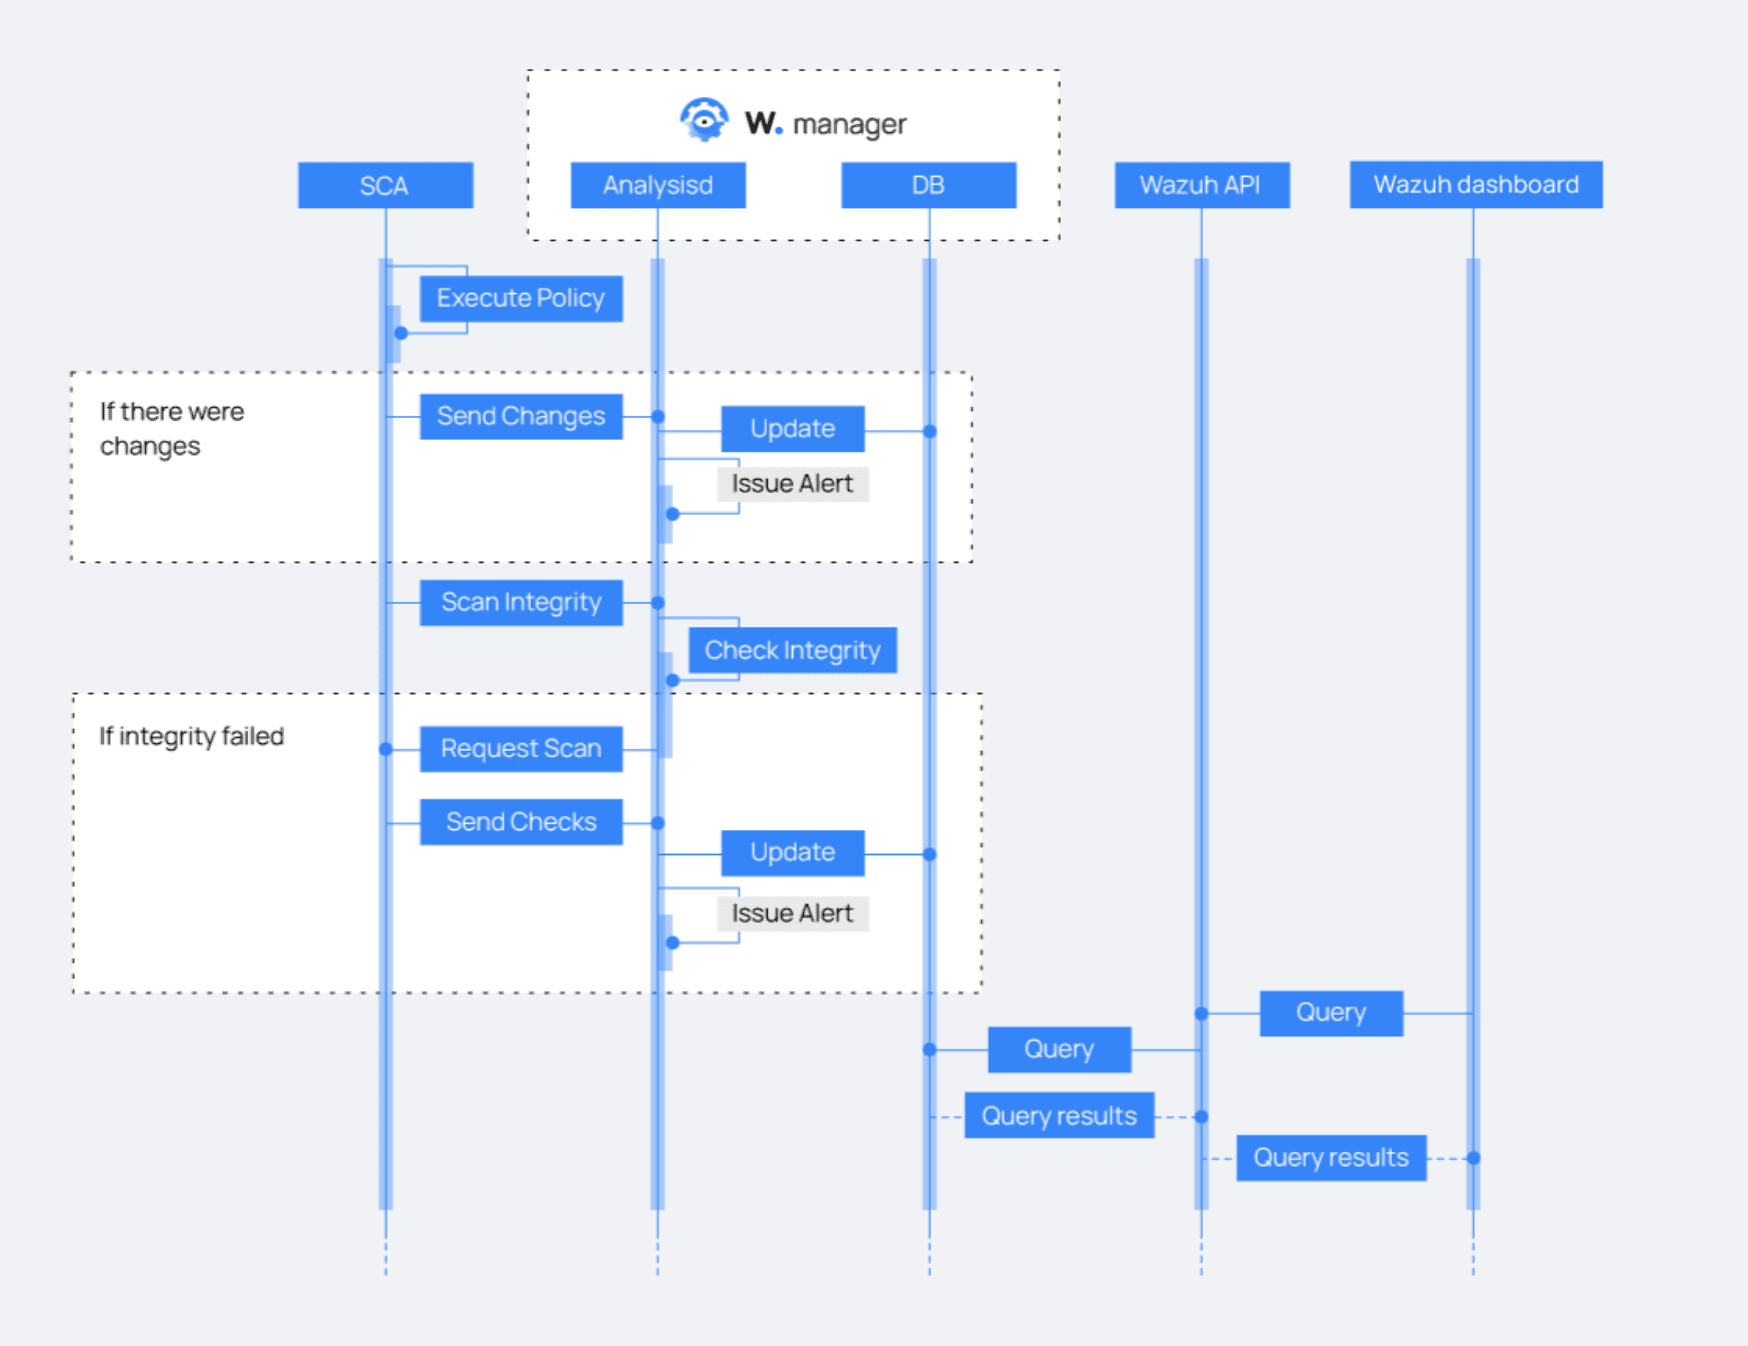
\includegraphics[width=\textwidth]{images/sca/sca-11.png}
    \caption{Integrity and Alerting Flow Diagram}
    \label{fig:sca-11}
\end{figure}

\paragraph{Overview of an SCA Check}
Checks are the core of an SCA policy, as they describe the scan to be performed in the endpoint. The checks contain fields that define what actions the agent should take to scan the endpoint, and how to evaluate the scan results. Each check definition comprises:

\begin{itemize}
    \item Metadata information including a rationale, remediation, and a description of the check.
    \item A logical description with the \texttt{condition} and \texttt{rules} fields.
\end{itemize}

As part of the metadata, the SCA policy can contain an optional compliance field used to specify if the check is relevant to any compliance specifications. SCA checks usually indicate standards or policies that they aim to comply with. For example, we map CIS benchmark, PCI-DSS, NIST, and TSC controls to the relevant SCA checks.

See below SCA policy ID \texttt{2651} for Debian 10 operating system as an example of a policy definition.
\begin{minted}{yaml}
- id: 2651
    title: "Ensure SSH HostbasedAuthentication is disabled"
    description: "The HostbasedAuthentication parameter specifies if authentication is allowed through trusted hosts via the user of .rhosts, or /etc/hosts.equiv, along with successful public key client host authentication. This option only applies to SSH Protocol Version 2."
    rationale: "Even though the .rhosts files are ineffective if support is disabled in /etc/pam.conf, disabling the ability to use .rhosts files in SSH provides an additional layer of protection."
    remediation: "Edit the /etc/ssh/sshd_config file to set the parameter as follows: HostbasedAuthentication no"
    compliance:
       - cis: ["5.2.9"]
       - cis_csc: ["16.3"]
       - pci_dss: ["4.1"]
       - hipaa: ["164.312.a.2.IV", "164.312.e.1", "164.312.e.2.I", "164.312.e.2.II"]
       - nist_800_53: ["SC.8"]
       - tsc: ["CC6.7"]
    condition: all
    rules:
       - 'c:sshd -T -> r:HostbasedAuthentication\s+no'
\end{minted}
\paragraph{Scan Results}
SCA scan results appear as alerts with SCA scan data whenever a particular check changes its status between scans. Moreover, Wazuh agents only send those events necessary to keep the global status of the scan updated, avoiding potential events flooding.

Any given check event has three possible results:
\begin{itemize}
    \item Passed
    \item Failed
    \item Not applicable
\end{itemize}

This result is determined by the set of rules and the rule result aggregator of the check.

Take the following SCA check from policy \texttt{cis\_debian10.yml} as an example. The example SCA check shown scans the Debian 10 endpoint to verify if you have implemented a “deny all” policy on your endpoint firewall:
\begin{minted}{yaml}
- id: 2603
    title: "Ensure IPv6 default deny firewall policy"
    description: "A default deny all policy on connections ensures that any unconfigured network usage will be rejected."
    rationale: "With a default accept policy the firewall will accept any packet that is not configured to be denied. It is easier to white list acceptable usage than to black list unacceptable usage."
    remediation: "Run the following commands to implement a default DROP policy: # ip6tables -P INPUT DROP # ip6tables -P OUTPUT DROP # ip6tables -P FORWARD DROP. Notes: Changing firewall settings while connected over network can result in being locked out of the system. Remediation will only affect the active system firewall, be sure to configure the default policy in your firewall management to apply on boot as well."
    compliance:
      - cis: ["3.5.4.2.1"]
      - cis_csc: ["9.4"]
      - pci_dss: ["1.2.1"]
      - tsc: ["CC8.1"]
    condition: all
    rules:
      - "c:ip6tables -L -> r:^Chain INPUT && r:policy DROP"
      - "c:ip6tables -L -> r:^Chain FORWARD && r:policy DROP"
      - "c:ip6tables -L -> r:^Chain OUTPUT && r:policy DROP"
\end{minted}

After evaluating the aforementioned check, the following event is generated:
\begin{minted}{yaml}
"data": {
  "sca": {
    "scan_id": "1433689708",
    "check": {
      "result": "failed",
      "remediation": "Run the following commands to implement a default DROP\
       policy: ip6tables -P INPUT DROP ip6tables -P OUTPUT DROP ip6tables \
       -P FORWARD DROP. Notes: Changing firewall settings while connected \
       over network can result in being locked out of the system. \
       Remediation will only affect the active system firewall, be sure \
       to configure the default policy in your firewall management to apply \
       on boot as well.",
      "compliance": {
        "pci_dss": "1.2.1",
        "tsc": "CC8.1",
        "cis_csc": "9.4",
        "cis": "3.5.4.2.1"
      },
      "description": "A default deny all policy on connections ensures that any unconfigured network usage will be rejected.",
      "id": "2603",
      "title": "Ensure IPv6 default deny firewall policy",
      "rationale": "With a default accept policy the firewall will accept any packet that is not configured to be denied. It is easier to white list acceptable usage than to black list unacceptable usage.",
      "command": [
        "ip6tables -L"
      ]
    },
    "type": "check",
    "policy": "CIS Benchmark for Debian/Linux 10"
  }
}
\end{minted}
You can view the scan summaries on the Security configuration assessment tab on the Wazuh dashboard.
\begin{figure} [H]
    \centering
    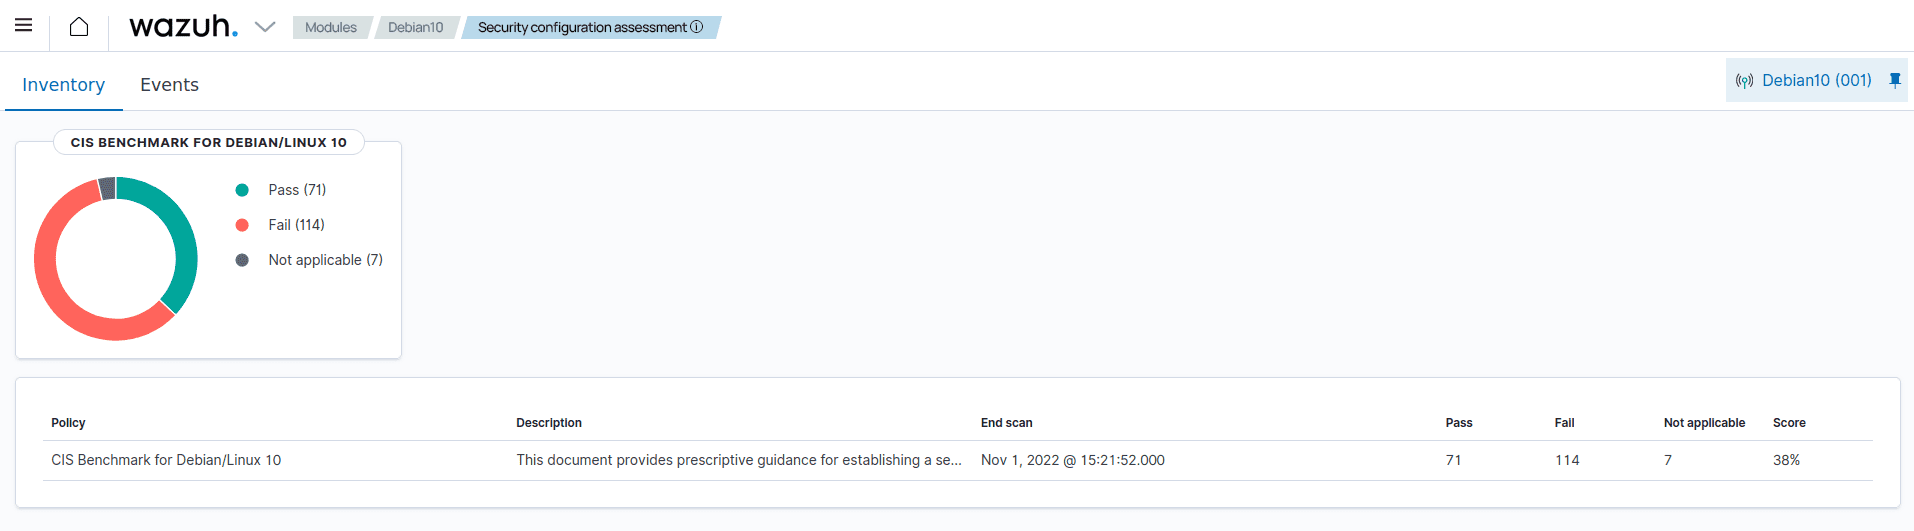
\includegraphics[width=0.5\textwidth]{images/sca/sca-12.png}
    \caption{Scan Summary on Security Configuration Assessment}
    \label{fig:sca-12}
\end{figure}

In addition, you can expand each result to display additional information.
\begin{figure} [H]
    \centering
    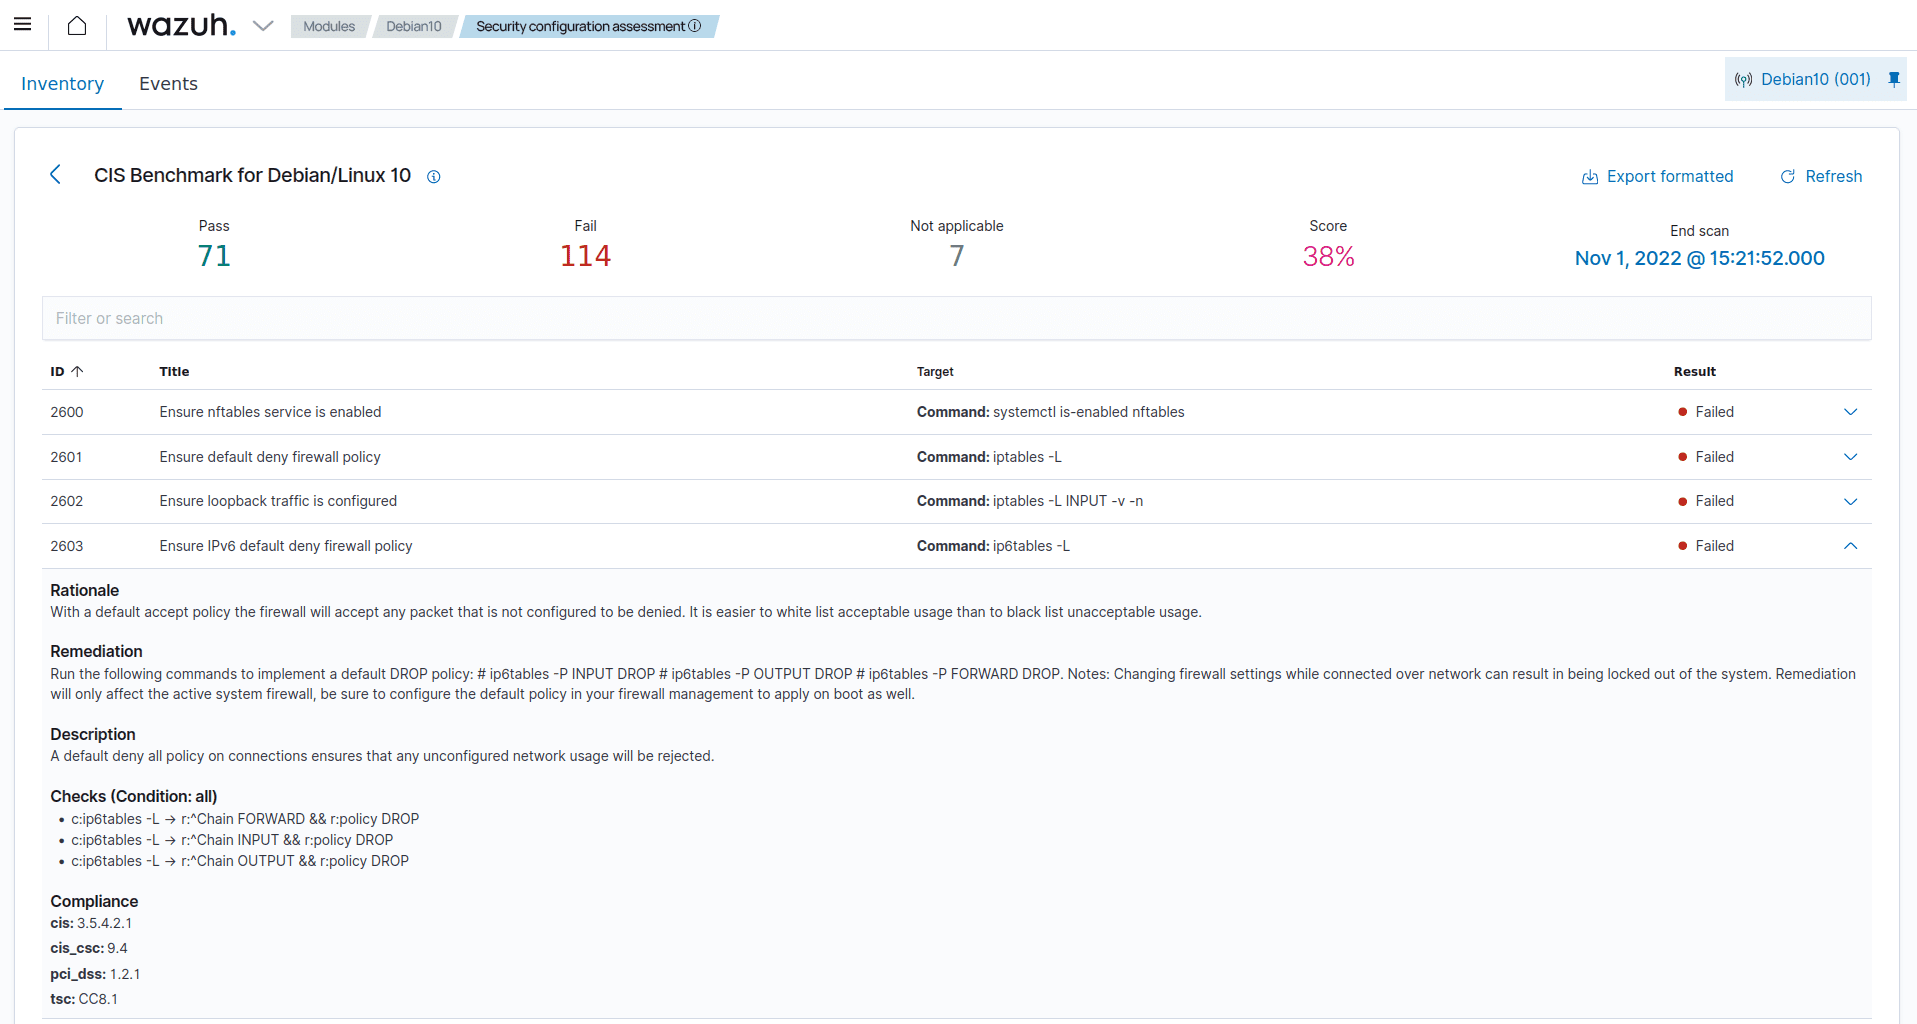
\includegraphics[width=\textwidth]{images/sca/sca-13.png}
    \caption{Expanded SCA Scan Result}
    \label{fig:sca-13}
\end{figure}

The above SCA scan result is Failed because the rule did not find Chain INPUT * policy DROP, Chain FORWARD * policy DROP, and Chain OUTPUT * policy DROP in the output of the command ip6tables \-L. The steps below show how we implement the remediation steps suggested by Wazuh to harden the endpoint:

\begin{itemize}
    \item Run the following recommended commands on the monitored endpoint to apply the firewall rules:
          \begin{minted}{bash}
ip6tables -P INPUT DROP
ip6tables -P OUTPUT DROP
ip6tables -P FORWARD DROP
    \end{minted}
    \item Save the firewall rules and make them persist on system reboot:
          \begin{minted}{bash}
ip6tables-save > /etc/ip6tables.conf
crontab -l | { cat; echo "@reboot /usr/sbin/ip6tables-restore /etc/ip6tables.conf"; } | crontab -
    \end{minted}
    \item Restart the Wazuh agent to trigger a new SCA scan:
          \begin{minted}{bash}
systemctl restart wazuh-agent
    \end{minted}
\end{itemize}
The scan result for check \texttt{2603} changes to Passed as shown in the image below:

\begin{figure} [H]
    \centering
    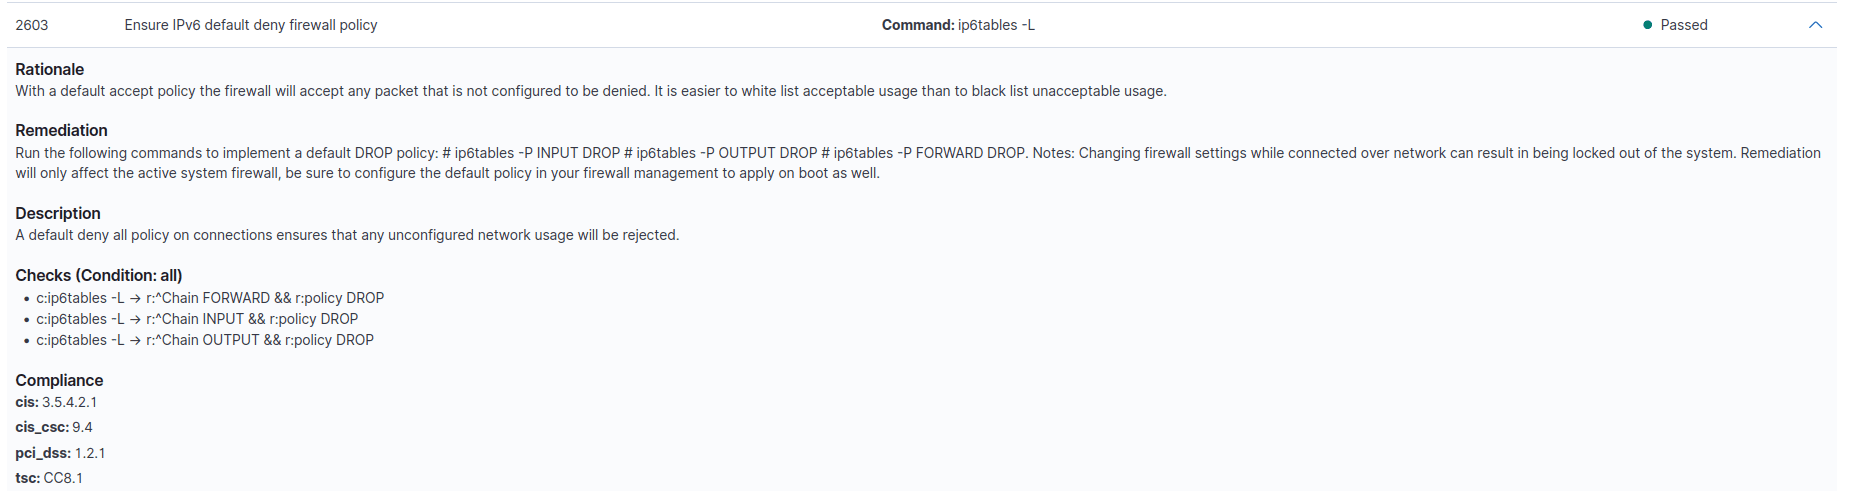
\includegraphics[width=\textwidth]{images/sca/sca-14.png}
    \caption{Scan Result for Check 2603}
    \label{fig:sca-14}
\end{figure}


SCA scan result
A check is marked as \texttt{Not applicable} in case an error occurs while performing the check. In such cases, instead of including the \texttt{result} field, the status and \texttt{reason} fields are included.

\paragraph{Integrity Mechanism}
Wazuh uses two integrity mechanisms to ensure integrity between agent-side and server-side SCA states. One of the integrity mechanisms ensures the integrity of the policy files and the second ensures the integrity of scan results.
\begin{itemize}
    \item Integrity of policy Files
    \item Integrity of Scan results
\end{itemize}

\subsubsection{Configuration}
Wazuh agents include the appropriate policies for their particular operating system during installation. For the full list of officially supported policy files, see the table Available SCA policies. These policies are included with the Wazuh server installation so that they can be easily enabled.

For a detailed description of the various configuration parameters of SCA, please check the SCA reference.

\paragraph{Enabling and Disabling Policies}
By default, the Wazuh agent runs scans for every policy (.yaml or .yml files) present in their ruleset folder:

\begin{itemize}
    \item Linux and Unix-based agents: \texttt{/var/ossec/ruleset/sca}.
    \item Windows agents: \texttt{C:\textbackslash Program Files (x86)\textbackslash ossec-agent\textbackslash ruleset\textbackslash sca}.
    \item macOS agents: \texttt{/Library/Ossec/ruleset/sca}.
\end{itemize}

To enable a policy file outside the Wazuh agent installation folder, add the policy file path to the \texttt{\textlangle sca\textrangle} block in the Wazuh agent configuration file. An example is shown below:

\begin{minted}{xml}
<sca>
    <policies>
        <policy><FULLPATH_TO_CUSTOM_SCA_POLICY_FILE></policy>
    </policies>
</sca>
\end{minted}

You can also specify a relative path to the Wazuh installation directory:

\begin{minted}{xml}
<sca>
    <policies>
        <policy>etc/shared/<CUSTOM_SCA_POLICY_FILE></policy>
    </policies>
</sca>
\end{minted}

There are two ways to disable policies on the Wazuh agent. The simplest one is renaming the policy file by adding .disabled (or anything different from .yaml or .yml) after their YAML extension.

The second is to disable them from the Wazuh agent ossec.conf file by adding a line such as the following to the <policy> section of the SCA module:

\begin{minted}{xml}
<sca>
    <policies>
        <policy enabled="no">etc/shared/<POLICY_FILE_TO_DISABLE></policy>
    </policies>
</sca>
\end{minted}

\paragraph{Sharing Policy Files and Configuration with the Wazuh Agents}
As described in the centralized configuration section, the Wazuh manager can push files and configurations to connected Wazuh agents.

You can enable this feature to push policy files to the Wazuh agents in defined groups. By default, every Wazuh agent belongs to the default group, which is used here as an example:

On the Wazuh agent, edit the \texttt{local\_internal\_options.conf} file to allow the execution of commands in SCA policies sent from the Wazuh server:


\begin{minted}{bash}
echo "sca.remote_commands=1" >> /var/ossec/etc/local_internal_options.conf
\end{minted}

On the Wazuh server, place a new policy file in the \texttt{/var/ossec/etc/shared/default} folder and change its ownership. Replace \texttt{<NEW\_POLICY\_FILE>} with your policy name.

\begin{minted}{bash}
chown wazuh:wazuh /var/ossec/etc/shared/default/<NEW\_POLICY\_FILE>
\end{minted}

Add the following configuration block to the Wazuh server /var/ossec/etc/shared/default/agent.conf file to configure the new policy file in the Wazuh agent:

\begin{minted}{xml}
<agent_config>
<!-- Shared agent configuration here -->
    <sca>
        <policies>
            <policy>etc/shared/<NEW_POLICY_FILE></policy>
        </policies>
    </sca>
</agent_config>
\end{minted}

All files remotely pushed from the Wazuh server are saved in the /<WAZUH\_HOME\_DIRECTORY>/etc/shared/ directory on the agent endpoints regardless of the group they belong to. We specify the relative file path of the policy in the configuration because the full file path could differ depending on the operating system of the monitored endpoint.

The new \texttt{<sca>} block in the Wazuh server \texttt{/var/ossec/etc/shared/default/agent}.conf file is merged with the \texttt{<sca>} block on the Wazuh agent side, and the new configuration is added.

\subsubsection{Simulation}
We demonstrate the use case of detecting a keyword in a file.
\paragraph{Detecting Keyword in a File}
In this use case, we demonstrate how you can configure Wazuh SCA to detect the presence of a keyword in a file. We monitor a file \texttt{testfile.txt} for the phrase \texttt{password\_enabled: yes}. The Wazuh SCA module triggers an alert when it detects the pattern in the file.
\subparagraph{Ubuntu endpoint}
\begin{itemize}
    \item We created the test file and add some text to it, including the phrase \texttt{password\_enabled: yes}.
          \begin{minted}{bash}
echo -e "config_file\nsecond line of configuration\npassword_enabled: yes" > /usr/share/testfile.txt
        \end{minted}

    \item We verified that the file was created and the phrase was present.
          \begin{minted}{bash}
cat /usr/share/testfile.txt
        \end{minted}
          Here is the output:
          \begin{figure} [H]
              \centering
              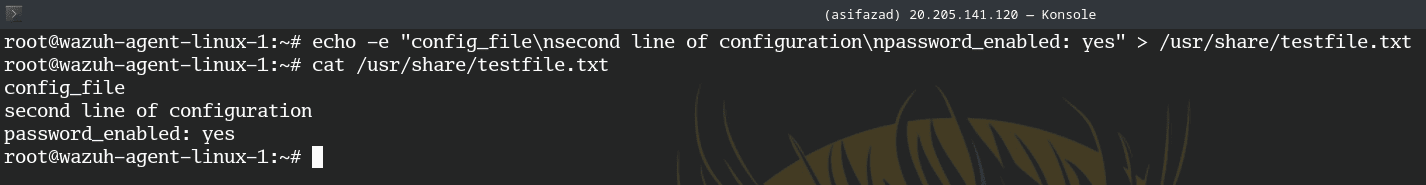
\includegraphics[width=\textwidth]{images/sca/sca-1.png}
              \caption{Creating the Test File and Adding the Phrase}
              \label{fig:sca-1}
          \end{figure}
    \item We created a new directory to save your custom policy files:
          \begin{minted}{bash}
mkdir /var/ossec/etc/custom-sca-files/
        \end{minted}

    \item We created a new SCA policy file \texttt{/var/ossec/etc/custom-sca-files/keywordcheck.yml} and add the following content to it:
        \begin{minted}{yaml}
policy:
  id: "keyword_check"
  file: "keywordcheck.yml"
  name: "SCA use case: Keyword check"
  description: "Guidance for checking for a keyword or phrase in files on Ubuntu endpoints."
  references:
    - https://documentation.wazuh.com/current/user-manual/capabilities/sec-config-assessment/index.html
    - https://documentation.wazuh.com/current/user-manual/capabilities/sec-config-assessment/creating-custom-policies.html

requirements:
  title: "Check that the desired file exists on the monitored endpoints"
  description: "Requirements for running the SCA scans against endpoints with testfile.txt on them."
  condition: any
  rules:
    - 'f:/usr/share/testfile.txt'

checks:
  - id: 10000
    title: "Ensure password is disabled in the test configuration file"
    description: "Password is enabled in the test configuration file."
    rationale: "Password is considered weak for the custom test application. Threat actors can brute-force your password."
    remediation: "Disable password by setting the value of the password_enabled option to no."
    condition: none
    rules:
      - 'f:/usr/share/testfile.txt -> r:^password_enabled: yes$'
        \end{minted}

    \item Change the ownership of the file so Wazuh has permission to it:
          \begin{minted}{bash}
chown wazuh:wazuh /var/ossec/etc/custom-sca-files/keywordcheck.yml
        \end{minted}


    \item We enabled the policy file by adding the following lines to the \texttt{<ossec\_config>} block of the Wazuh agent configuration file at \texttt{/var/ossec/etc/ossec.conf}
          \begin{figure} [H]
              \centering
              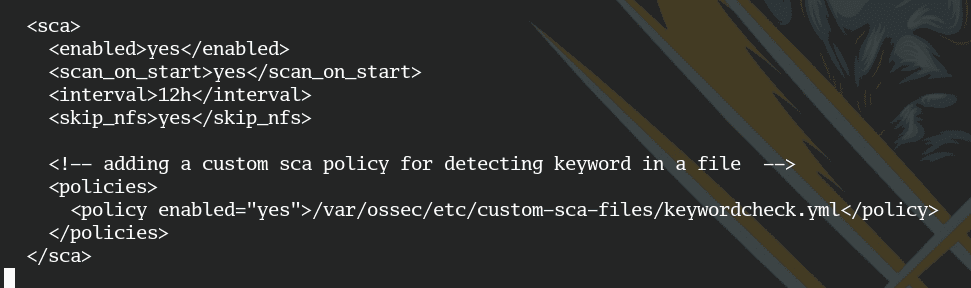
\includegraphics[width=\textwidth]{images/sca/sca-3.png}
              \caption{Enabling the Policy File}
              \label{fig:sca-3}
          \end{figure}

    \item Restart the Wazuh agent to apply the changes and to run the new SCA check:
          \begin{minted}{bash}
systemctl restart wazuh-agent
        \end{minted}

    \item All the steps in terminal.
          \begin{figure} [H]
              \centering
              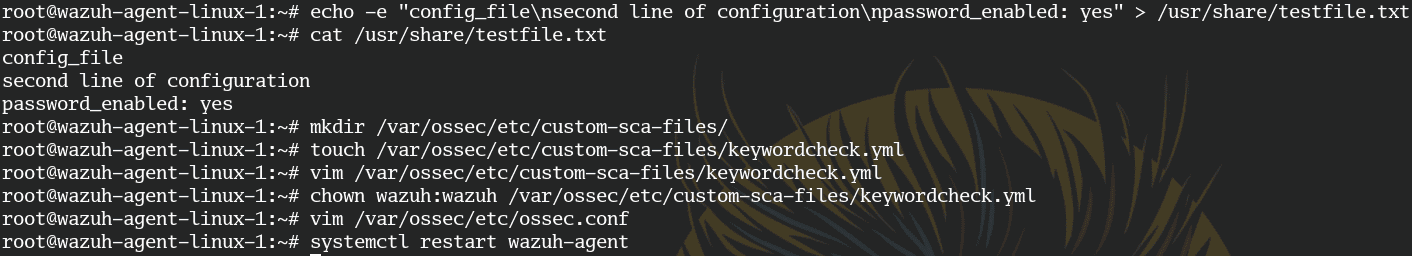
\includegraphics[width=\textwidth]{images/sca/sca-4.png}
              \caption{All the Steps in Terminal}
              \label{fig:sca-4}
          \end{figure}

\end{itemize}

\subsubsection{Dashboard Update}
\paragraph{Detecting Keyword in a File}
On our Wazuh dashboard, we navigated to the SCA tab and selected the Ubuntu endpoint to view the results of the custom SCA check we have created.
\begin{figure} [H]
    \centering
    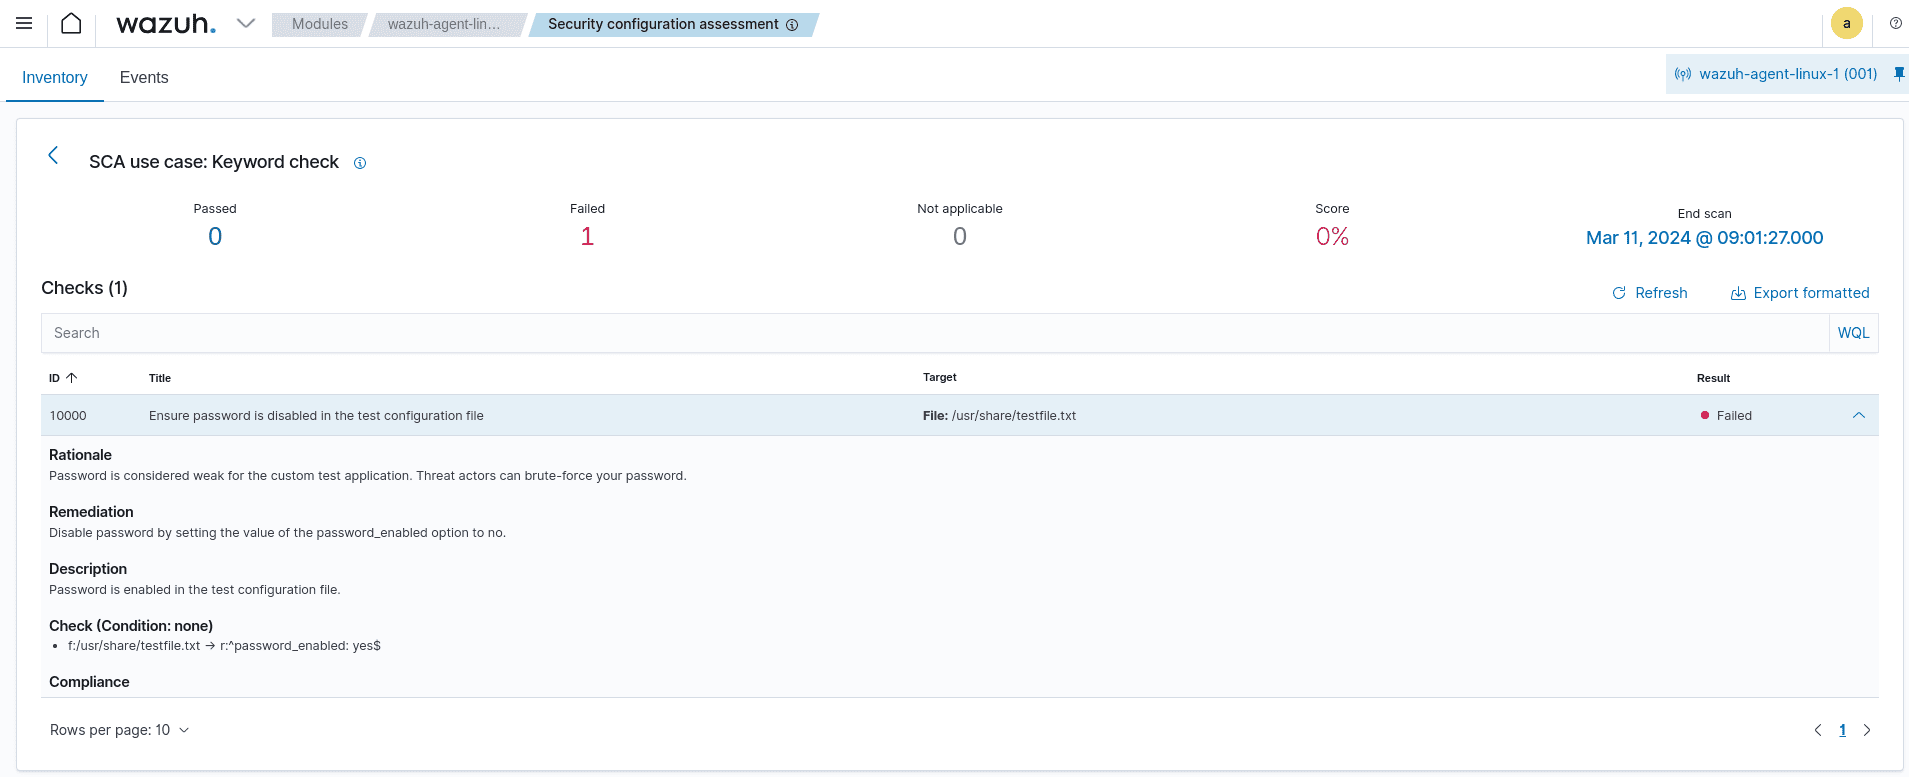
\includegraphics[width=0.65\textwidth]{images/sca/sca-5.png}
    \caption{Dashboard Update for the Custom SCA Check}
    \label{fig:sca-5}
\end{figure}


